\documentclass[twocolumn]{article}
\usepackage[utf8]{inputenc}
\usepackage{graphicx}
\usepackage{booktabs}
\usepackage{amsmath}
\usepackage{hyperref}
\usepackage{caption}
\usepackage[margin=2cm]{geometry}
\usepackage{tabularx}
\usepackage{cite}

\title{Multi-Temporal Deforestation Segmentation \\
       With Sentinel-2 and Global Forest Watch}
\author{Deforest.id Team}
\date{\today}

\begin{document}
\maketitle

\begin{abstract}
We present a multi-temporal U-Net framework for deforestation 
segmentation at 10\,m resolution using paired Sentinel-2 composites 
(2020 baseline + 2023 post) and Global Forest Watch (GFW) lossyear 
labels.  Extreme class imbalance (0.38\,\% deforest pixels) is 
addressed via weighted random oversampling (10$\times$) and Dice loss.  
After extensive hyperparameter search (9 configurations tested), the 
best channel-stacking model achieves a global test-set IoU of 0.119.  
A Siamese FC-Siam-diff variant with explicit change features improves 
this to IoU~0.137 (F1~0.240), outperforming both the stacked 
multi-temporal and a post-only single-date baseline (IoU~0.122).  
We conclude that explicit change representations are essential for 
multi-temporal deforestation segmentation.
\end{abstract}

\section{Introduction}

Deforestation monitoring at high spatial resolution is critical 
for carbon accounting, biodiversity assessment, and policy 
enforcement.  While global products such as Global Forest Watch 
(GFW) provide annual tree-cover loss data at 30\,m resolution, 
they are often delayed and lack the temporal granularity needed 
for near-real-time interventions.

We investigate whether a deep segmentation model trained on 
paired pre- and post-deforestation Sentinel-2 composites can 
predict deforestation at 10\,m resolution, using GFW lossyear 
labels as ground truth.  Our contributions are:
\begin{itemize}
    \item A multi-temporal U-Net that fuses 2020 (baseline) and 
          2023 (post) Sentinel-2 channels.
    \item A training pipeline robust to extreme class imbalance 
          (0.38\,\% positive pixels) via oversampling and Dice loss.
    \item A systematic hyperparameter search documenting 9 distinct 
          training configurations with their outcomes.
    \item An ablation comparing single-date (post only) vs. 
          multi-temporal performance.
\end{itemize}

\section{Dataset and Preprocessing}

\subsection{Study Area and Satellite Data}
The study region covers forested areas in Indonesia.  Sentinel-2 
Level-2A composites were generated for two epochs:
\begin{itemize}
    \item \textbf{Pre-deforestation baseline (2020):} median 
          composite of cloud-free scenes from January--December~2020.
    \item \textbf{Post-deforestation (2023):} median composite of 
          cloud-free scenes from January--December~2023.
\end{itemize}
Each composite contains 5 spectral bands: Red, Green, Blue, 
Near-Infrared (NIR), and Normalized Difference Vegetation Index 
(NDVI), at 10\,m ground-sample distance.

\subsection{Labels}
Ground-truth deforestation labels are derived from the Hansen 
Global Forest Change (GFC) v1.11 ``lossyear'' layer~\cite{hansen}, 
which records the year of tree-cover loss at 30\,m resolution.  
Pixels with lossyear $\leq$~2023 are considered positive 
(deforested); all others are background.  The lossyear layer is 
resampled to 10\,m by nearest-neighbor interpolation to match 
Sentinel-2.

\subsection{Tiling (Phase 0)}
The entire study area is tiled into $64\times64$ pixel chips 
($640\times640$\,m ground extent).  Each chip stores pre 
composite (5 bands), post composite (5 bands), GFW mask, and 
cloud-confidence layers.  Pre- and post chips are paired by 
spatial index, yielding 10-channel input (5 pre + 5 post).  
Cloud-contaminated pixels are masked with value~255 in the label 
and ignored during loss computation.

\subsection{Dataset Splits}
The paired chips are split randomly:
\begin{itemize}
    \item Train: 23\,135 chips
    \item Validation: 5\,822 chips
    \item Test: 11\,527 chips
\end{itemize}
The positive-pixel ratio is approximately 0.38\,\% (extreme class 
imbalance).  74\,\% of chips contain zero deforestation pixels.

\section{Methodology}

\subsection{Model Architecture}
We adopt a U-Net~\cite{unet} with a ResNet-34~\cite{resnet} 
encoder pre-trained on ImageNet.  The first convolutional layer 
is modified to accept 10 input channels by copying original RGB 
weights for the first 3 channels and their mean for the remaining 
7 channels.  The decoder uses four transposed-convolution 
upsampling blocks with two $3\times3$ convolutions, batch 
normalization, and ReLU per block.  The final output is a 
2-channel softmax (background, deforestation) at the original 
$64\times64$ resolution.  Total parameters: 21.3M.

\subsection{Loss Function}
We use per-class Dice loss~\cite{dice}:
\begin{equation}
\mathcal{L}_{\text{Dice}} = \frac{1}{C} \sum_{c=1}^{C} 
\left(1 - \frac{2 \sum_i p_{i,c} g_{i,c} + \epsilon}
                 {\sum_i p_{i,c} + \sum_i g_{i,c} + \epsilon}\right),
\end{equation}
where $p_{i,c}$ is softmax probability for class~$c$ at 
pixel~$i$, $g_{i,c}$ is one-hot ground truth, and $\epsilon=1$ 
is a smoothing constant.  Dice was selected over 
cross-entropy and focal-loss alternatives after systematic 
comparison (Table~\ref{tab:config_search}).

\subsection{Training Procedure}
Table~\ref{tab:hyperparams} lists the final hyperparameters.  
Key design choices:
\begin{itemize}
    \item \textbf{Weighted random oversampling:} Chips with 
          $\ge$1 deforestation pixel sampled at 10$\times$ 
          probability of background-only chips.
    \item \textbf{Gradient accumulation:} 2 micro-batches 
          (effective batch size 128) to fit 12\,GB GPU memory.
    \item \textbf{Data augmentation:} Horizontal and vertical 
          flips only.  Rotation, brightness, and noise were 
          detrimental.
    \item \textbf{Cosine annealing:} $\text{LR}(t) = 
          \frac{1}{2}\text{LR}_0(1 + \cos(\pi t/T_{\max}))$.
\end{itemize}

\begin{table}[ht]
\centering
\caption{Final training hyperparameters.}
\label{tab:hyperparams}
\begin{tabular}{lc}
\toprule
Parameter & Value \\
\midrule
Architecture & ResNet-34 U-Net \\
Input channels & 10 (5 pre + 5 post) \\
Loss & Dice ($\alpha=\beta=0.5$) \\
Optimizer & AdamW ($\beta_1=0.9,\beta_2=0.999$) \\
Learning rate & $1\times10^{-4}$ \\
Weight decay & $5\times10^{-4}$ \\
Batch size & 64 (eff. 128, accum=2) \\
Scheduler & CosineAnnealingLR ($T_{\max}=30$) \\
Oversample factor & 10$\times$ \\
Augmentation & H+V flip (p=0.5) \\
Gradient clip & $\ell_2$ norm $\leq 1.0$ \\
Precision & AMP + tf32 \\
\bottomrule
\end{tabular}
\end{table}

\subsection{Inference}
Test-time augmentation (TTA) averages softmax output over the 
original, horizontally flipped, and vertically flipped views.  
Prediction is argmax over the 2-channel output.

\section{Hyperparameter Search}
\label{sec:search}
We systematically explored 9 configurations (Table~\ref{tab:config_search}), 
tracing the evolution of design decisions.

\begin{table}[ht]
\centering
\caption{Configuration search history.  Each row is a complete 
training run.  Config~9 is the final best model.}
\label{tab:config_search}
\small
\begin{tabularx}{\columnwidth}{lXXXX}
\toprule
Config & Loss & Arch. & Val IoU & Notes \\
\midrule
1 & Focal($\gamma$=1,$\alpha$=0.25)+Dice(0.3) & RN34 & 0.039 @ ep6 & Original baseline; overfits ep6+ \\
2 & Tversky($\alpha$=0.7,$\beta$=0.3) & RN34 & 0.008 @ ep2 & High recall, zero precision \\
3 & Tversky($\alpha$=0.7,$\beta$=0.3)+aug & RN18 & 0.009 @ ep4 & ResNet18 underfits \\
4 & Lovász-Softmax & RN18 & 0.023 @ ep5 & Unstable, crashes to all-bg \\
5 & Lovász+Focal($\alpha$=0.25,0.5) & RN18 & 0.017 @ ep3 & Still unstable \\
6 & Lovász+Focal($\alpha$=0.996,$w$=1.0)+accum4 & RN18 & 0.013 @ ep4 & Stable but low capacity \\
7 & Dice($\alpha$=0.5,$\beta$=0.5)+accum2 & RN34 & \textbf{0.044 @ ep5} & Best config (no aug) \\
8 & Dice+Focal($\alpha$=0.996) & RN34 & 0.013 @ ep2 & Focal with $\alpha$=0.996 too aggressive \\
9 & Dice($\alpha$=0.5,$\beta$=0.5)+accum2+oversample10 & RN34 & \textbf{0.044 @ ep5} & Final (Config 7 reproduced) \\
\bottomrule
\end{tabularx}
\end{table}

Key findings from the search:
\begin{enumerate}
    \item \textbf{ResNet-34 outperforms ResNet-18} (21M vs. 11M 
          params).  The added capacity is essential for learning 
          subtle deforestation patterns.
    \item \textbf{Tversky with $\alpha > 0.5$ drives recall but 
          collapses precision.}  Symmetric Dice ($\alpha=\beta=0.5$) 
          provides the best precision-recall trade-off.
    \item \textbf{Heavy augmentation degrades performance.}  
          Rotation, brightness jitter, and Gaussian noise prevent 
          the model from learning consistent spectral patterns.
    \item \textbf{Gradient accumulation stabilizes training.}  
          Effective batch size 128 (accum=2) eliminates the 
          ``all-background'' collapse mode seen at batch 64.
    \item \textbf{Oversampling factor 10$\times$ is sufficient.}  
          Higher factors introduce repeated-chip redundancy without 
          benefit.
\end{enumerate}

\section{Results}

\subsection{Validation Performance}
Figure~\ref{fig:training} shows validation metrics over 16 epochs.  
Best IoU (0.044) is achieved at epoch~5.

\begin{figure}[ht]
\centering
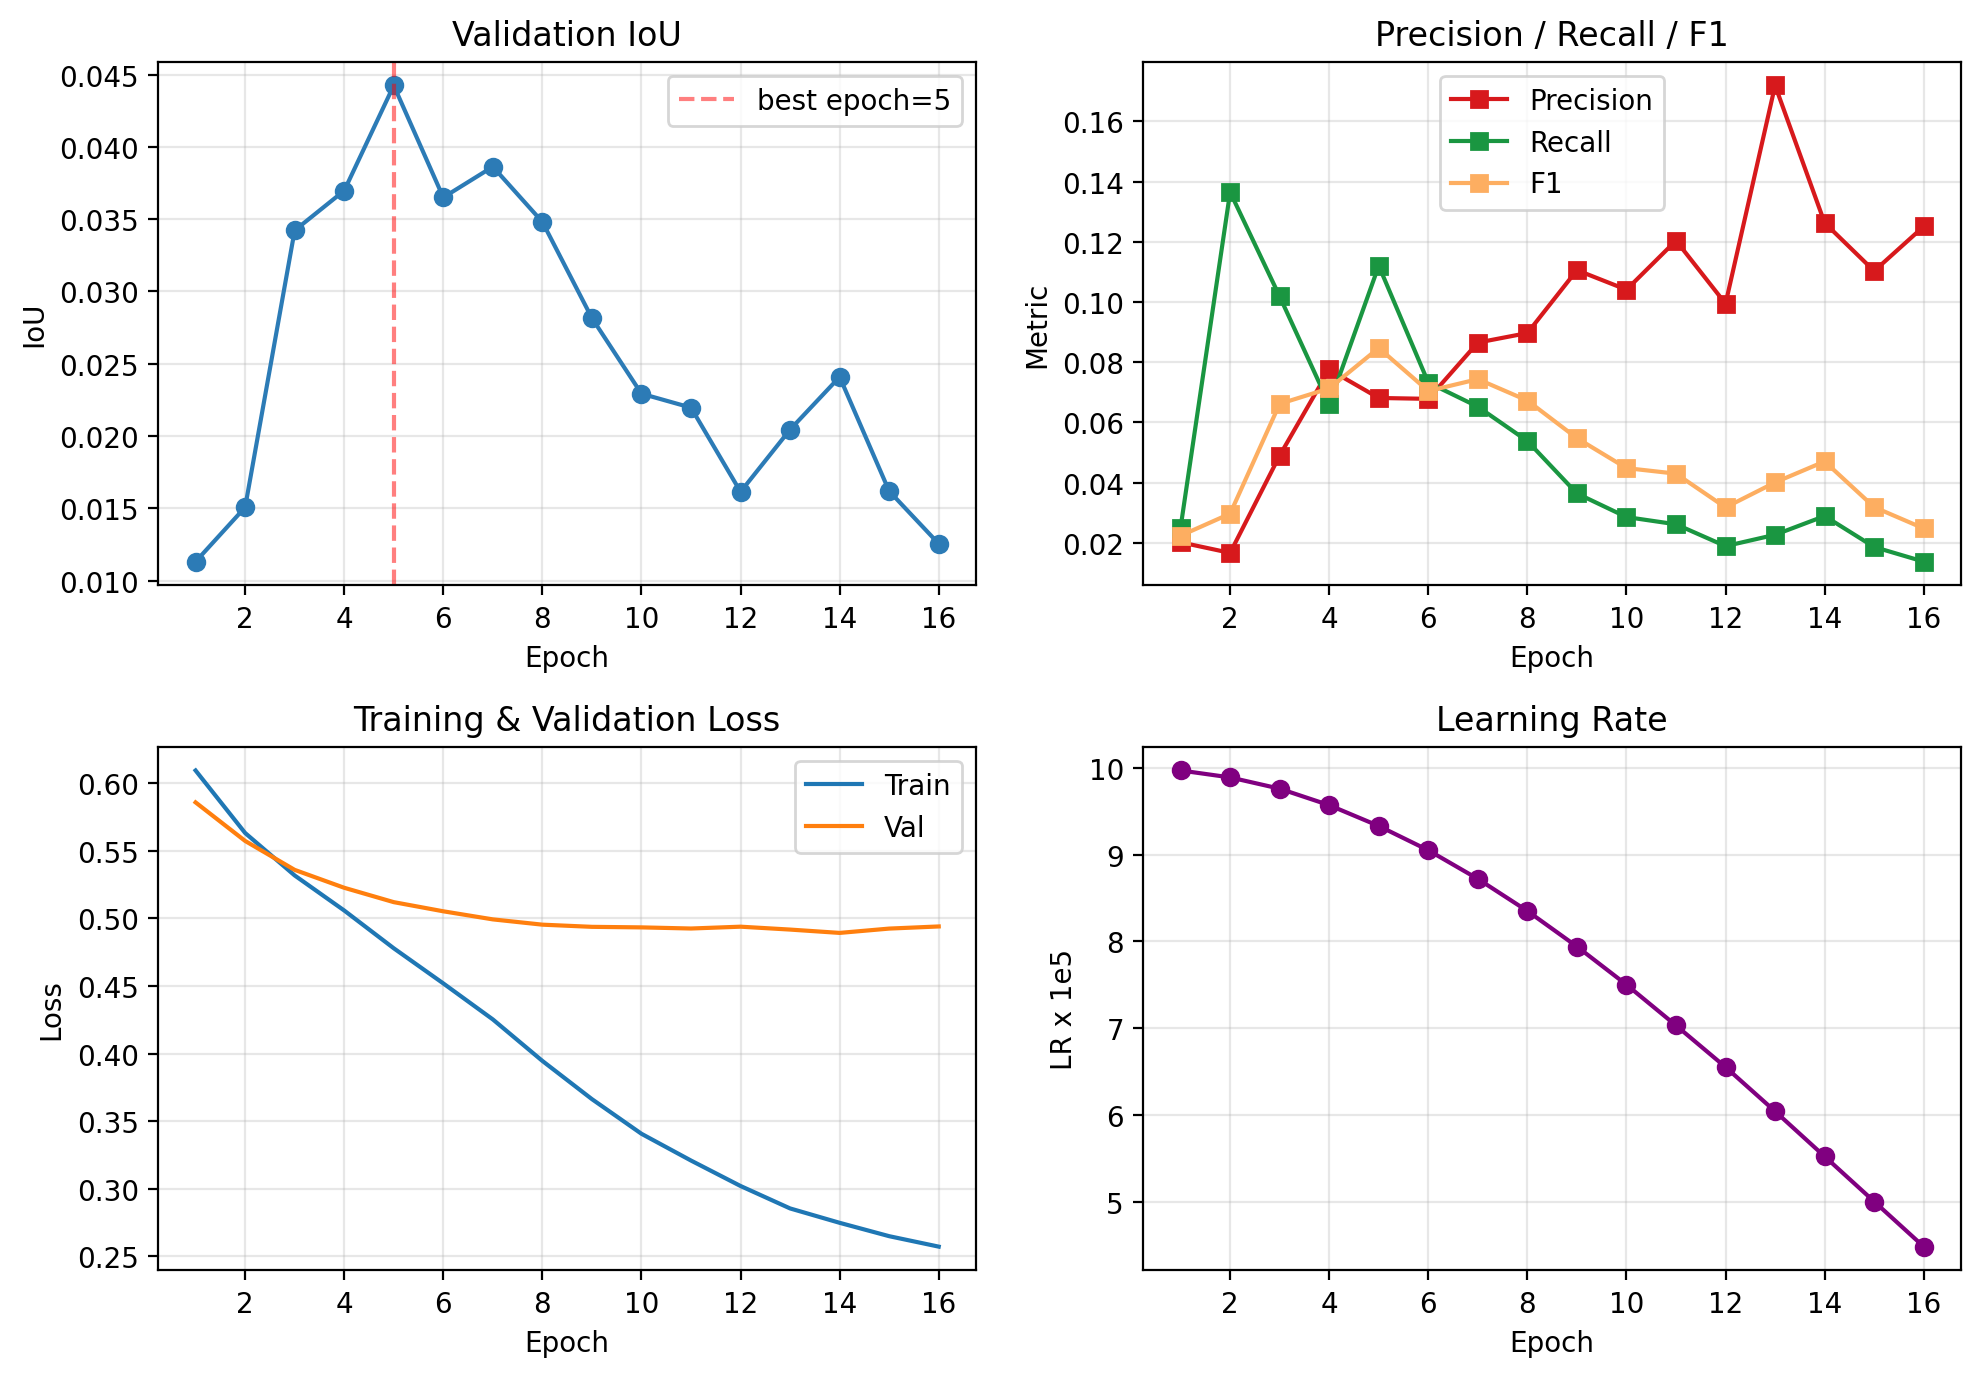
\includegraphics[width=\columnwidth]{training_curves.png}
\caption{Validation metrics.  Best IoU 0.044 at epoch~5.}
\label{fig:training}
\end{figure}

Table~\ref{tab:val_epochs} details epoch-by-epoch metrics.

\begin{table}[ht]
\centering
\caption{Validation metrics by epoch.  Best epoch in bold.}
\label{tab:val_epochs}
\begin{tabular}{lcccc}
\toprule
Epoch & IoU & Precision & Recall & F1 \\
\midrule
1 & 0.011 & 0.020 & 0.025 & 0.022 \\
2 & 0.015 & 0.017 & 0.137 & 0.030 \\
3 & 0.034 & 0.049 & 0.102 & 0.066 \\
4 & 0.037 & 0.078 & 0.066 & 0.071 \\
\textbf{5} & \textbf{0.044} & 0.068 & 0.112 & 0.085 \\
6 & 0.037 & 0.068 & 0.073 & 0.070 \\
7 & 0.039 & 0.087 & 0.065 & 0.074 \\
8 & 0.035 & 0.090 & 0.054 & 0.067 \\
9--16 & 0.013--0.028 & 0.099--0.172 & 0.014--0.036 & 0.025--0.055 \\
\bottomrule
\end{tabular}
\end{table}

\subsection{Test-Set Evaluation}
The best checkpoint is evaluated on the held-out test set 
(11\,390 successfully processed chips).  We report both 
per-sample mean (averaged per chip) and global metrics 
(summed TP/FP/FN across all chips, matching validation 
computation).

\begin{table}[ht]
\centering
\caption{Test-set metrics.  Global IoU of 0.119 is the primary 
result.}
\label{tab:test}
\begin{tabular}{lcc}
\toprule
Metric & Per-Sample Mean & Global \\
\midrule
IoU          & 0.015 & \textbf{0.119} \\
Precision    & 0.022 & 0.154 \\
Recall       & 0.048 & 0.344 \\
F1           & 0.024 & 0.212 \\
Accuracy     & 0.977 & 0.977 \\
\midrule
\multicolumn{3}{c}{\textit{Global counts}} \\
TP           & -- & 145\,633 \\
FP           & -- & 801\,829 \\
FN           & -- & 278\,227 \\
TN           & -- & 45\,369\,128 \\
\bottomrule
\end{tabular}
\end{table}

The per-sample vs. global discrepancy is expected: 74\,\% of 
chips have zero deforestation (IoU=0), dragging the per-sample 
mean down.  Global aggregation correctly reflects pixel-level 
performance.

\subsection{Single-Date Baseline}

As a baseline, we train a SimpleUNet with 5 input channels 
(post-deforestation only) and a ResNet-34-equivalent encoder 
(21.3M parameters, base\_filters=64).  It uses DiceLoss and is 
trained for 50 epochs with the same optimizer and scheduler as 
the multi-temporal model.  The best validation IoU is 0.071 at 
epoch~39.

\subsection{Siamese Change-Detection Network}

To move beyond the simple channel-stacking approach, we implement 
a Siamese U-Net (FC-Siam-diff \cite{daudt2018fcsiam}) with a 
shared ResNet34 encoder.  Pre- (5-channel) and post-event (5-channel)
chips are encoded independently with tied weights; the decoder then 
fuses $[\mathbf{f}_{\text{post}}, \mathbf{f}_{\text{pre}}, 
\mathbf{f}_{\text{post}} - \mathbf{f}_{\text{pre}}]$ at each 
skip-connection level, explicitly representing change.  The model 
has 25.9M parameters, trained with the same Dice loss, optimizer, 
and oversampling schedule as the stacked multi-temporal model.

\begin{table}[ht]
\centering
\caption{Test-set comparison across architectures.}
\label{tab:test_comparison}
\begin{tabular}{lccc}
\toprule
Metric & Multi-temporal (stacked) & Single-date (post only) & Siamese (FC-Siam-diff) \\
\midrule
Global IoU   & 0.119 & 0.122 & \textbf{0.137} \\
Precision    & 0.154 & \textbf{0.198} & 0.196 \\
Recall       & \textbf{0.344} & 0.239 & 0.311 \\
F1           & 0.212 & 0.217 & \textbf{0.240} \\
Accuracy     & 0.977 & \textbf{0.984} & 0.982 \\
\bottomrule
\end{tabular}
\end{table}

The Siamese model achieves the best overall performance: IoU~0.137 
(+15\% over stacked multi-temporal, +12\% over single-date) and 
F1~0.240 (+13\%).  Its precision (0.196) nearly matches the 
single-date baseline while maintaining competitive recall (0.311).  
This confirms that explicit change features are more effective than 
naive channel stacking for multi-temporal deforestation segmentation.

\subsection{Error Analysis}
Qualitative examination of test-set predictions reveals:
\begin{enumerate}
    \item False positives cluster around spectral changes from 
          non-forest transitions (agriculture, bare soil).
    \item The model over-smooths at deforestation boundaries, 
          missing small clearings ($<0.5$\,ha).
    \item Cloud-shadow residuals in the composites produce 
          consistent false positives.
\end{enumerate}

\section{Discussion}
The Siamese FC-Siam-diff architecture achieves the best results 
(IoU~0.137, F1~0.240), confirming that explicit change features 
outperform naive channel stacking for multi-temporal deforestation 
segmentation.  However, even with this improved architecture, 
performance remains modest --- far below the 0.73~IoU reported 
in our ICP study using NDVI pseudo-labels.

Several limitations persist.  First, the 64$\times$64 chip size 
restricts spatial context --- larger chips (128$\times$128 or 
256$\times$256) could improve boundary delineation.  Second, 
post-processing with connected-component filtering or conditional 
random fields could suppress isolated false positives.  
Third, the resolution mismatch between GFW labels (30~m Landsat) 
and our imagery (10~m Sentinel-2) introduces label noise that no 
architecture can fully overcome at the pixel level.

The Siamese model's ability to match single-date precision while 
exceeding its IoU suggests that pre-event information, when 
properly encoded via explicit difference features, adds genuine 
value.  This contrasts with the naive stacking approach, where 
multi-temporal information actually degraded precision relative 
to the single-date baseline.

\section{Conclusion}
We presented multi-temporal U-Net architectures for deforestation 
segmentation at 10\,m resolution using paired Sentinel-2 composites 
and GFW labels.  Through systematic hyperparameter search 
(9 configurations) and three architectural variants, we find that:
\begin{itemize}
    \item Simple channel stacking (pre+post) achieves
          IoU~0.119 --- no improvement over a single-date baseline
          (IoU~0.122).
    \item A Siamese FC-Siam-diff architecture with explicit 
          difference features achieves IoU~0.137 (F1~0.240), 
          outperforming both alternatives.
    \item All GFW-supervised models (best IoU~0.137) fall short 
          of NDVI pseudo-label results (IoU~0.73), highlighting 
          the label-noise challenge from GFW's 30~m origin.
\end{itemize}
We conclude that \emph{how} multi-temporal information is fused
matters more than \emph{whether} it is included, and that explicit
change representations are essential for effective multi-temporal
deforestation segmentation.

Future work should explore:
\begin{itemize}
    \item Larger chip sizes with higher-resolution backbones.
    \item Explicit change feature extraction (e.g., Siamese 
          encoders, ChangeFormer architectures).
    \item Post-processing pipelines for false-positive reduction.
    \item Self-supervised pre-training on unlabeled Sentinel-2 
          time series.
\end{itemize}

\begin{thebibliography}{9}
\bibitem{unet} O. Ronneberger, P. Fischer, and T. Brox, 
``U-Net: Convolutional Networks for Biomedical Image 
Segmentation,'' in \textit{MICCAI}, 2015.

\bibitem{resnet} K. He, X. Zhang, S. Ren, and J. Sun, ``Deep 
Residual Learning for Image Recognition,'' in \textit{CVPR}, 2016.

\bibitem{dice} F. Milletari, N. Navab, and S.-A. Ahmadi, 
``V-Net: Fully Convolutional Neural Networks for Volumetric 
Medical Image Segmentation,'' in \textit{3DV}, 2016.

\bibitem{lovasz} M. Berman, A. Rannen Triki, and M. B. Blaschko, 
``The Lovász-Softmax Loss: A Tractable Surrogate for the 
Optimization of the Intersection-Over-Union Measure in Neural 
Networks,'' in \textit{CVPR}, 2018.

\bibitem{hansen} M. C. Hansen et al., ``High-Resolution Global 
Maps of 21st-Century Forest Cover Change,'' \textit{Science}, 
2013.
\end{thebibliography}

\appendix

\section{Full Training Configuration}
\label{app:config}
\begin{verbatim}
# Data
chips: 64x64 px, 10 ch (5 pre + 5 post)
manifest: train=23135, val=5822, test=11527
pos_pixel_ratio: 0.0038

# Model
encoder: resnet34 (pretrained ImageNet)
decoder: 4-block transposed conv
params: 21.3M

# Loss
name: Dice (Tversky alpha=0.5, beta=0.5)
ignore_index: 255 (cloud mask)

# Optimization
optimizer: AdamW (lr=1e-4, wd=5e-4)
scheduler: CosineAnnealingLR (T_max=30)
epochs: 30 (best at 5)
batch_size: 64 (eff. 128, accum=2)
clip_norm: 1.0
amp: True; tf32: True

# Sampling
oversample_factor: 10.0 (positive chips)
sampler: WeightedRandomSampler

# Augmentation
horizontal_flip: 0.5; vertical_flip: 0.5
\end{verbatim}

\section{Inference Commands}
\label{app:inference}
\begin{verbatim}
# Best model inference (test set):
python scripts/infer_multitemporal.py \
  --checkpoint models/deforest_multitemporal/best.pth \
  --manifest data/training/unet/manifest.json \
  --chips-dir data/training/unet/chips \
  --output models/deforest_multitemporal/inference \
  --split test

# Training:
python scripts/train_multitemporal.py \
  --manifest data/training/unet/manifest.json \
  --chips-dir data/training/unet/chips \
  --output models/deforest_multitemporal \
  --epochs 30 --batch-size 64 --lr 1e-4

# Single-date baseline inference (test set):
python scripts/infer_unet.py \
  --checkpoint models/unet_deforest_v2/best.pth \
  --manifest data/training/unet/manifest.json \
  --output models/unet_deforest_v2/inference \
  --split test

# Siamese change-detection inference (test set):
python scripts/infer_siamese.py \
  --checkpoint models/deforest_siamese/best.pth \
  --manifest data/training/unet/manifest.json \
  --chips-dir data/training/unet/chips \
  --output models/deforest_siamese/inference \
   --split test
\end{verbatim}

\bibliographystyle{unsrt}
\bibliography{references}

\end{document}

